\pgfplotsset{width=15cm,compat=1.9}

\pgfplotsset{
  log ticks with fixed point,
}
% \begin{tikzpicture}
%     \begin{semilogxaxis}[
%         title={Transformer benchmark fp32 WASM versus WebGPU},
%         xlabel={Aantal parameters in miljoen},
%         ylabel={Uitvoeringstijd in ms},
%         xmin=38, xmax=1551,
%         ymin=0, ymax=120,
%         xtick={39, 74, 244, 769, 1550},
%         legend pos=north west,
%         ymajorgrids=true,
%         grid style=dashed,
%         scatter/classes={
%             a={mark=square*,red},
%             b={mark=triangle*,orange},
%             c={mark=square,green}
%         },
%         yticklabel style={
%             /pgf/number format/fixed,
%         },
%         scaled y ticks=false
%     ]
%         \addplot [
%             scatter,only marks,
%             scatter src=explicit symbolic,
%         ] table [x=x,y=y,meta=label] {plotdata/whispertest.dat};

%     \end{semilogxaxis}
% \end{tikzpicture}

% \begin{tikzpicture}
%     \begin{axis}[
%         title={Whisper met CUDA en CPU},
%         xmin=0, xmax=4,
%         xtick={1,2,3},
%         ymin=0, ymax=60000,
%         % x tick label style={
%         %     /pgf/number format/1000 sep=},
%         ylabel=ms,
%         enlargelimits=0.05,
%         legend style={at={(0.5,-0.1)},
%         anchor=north,legend columns=-1},
%         % ybar interval=0.7,
%     ]
%         \addplot 
%             coordinates {(1, 17602.3325)(1, 17063.286)(1, 17377.5252)(1, 17397.9507)(1, 17456.7227)(1, 17513.7898)};
%         \addplot 
%             coordinates {(2, 34039.00)(2, 34735.00)(2, 34572.00)(2, 34290.00)(2, 34231.00)(2, 34697.00)};
%         \addplot 
%             coordinates {(3, 57788.052)(3, 58644.8482)(3, 58614.227)(3, 58611.5474)(3, 59072.5315)(3, 58373.3585)};
%         \legend{CUDA - Nvidia Geforce GTX 1080 Ti,CPU - Intel Core i9,CPU - Xeon E5-2680 V2}
%     \end{axis}
% \end{tikzpicture}

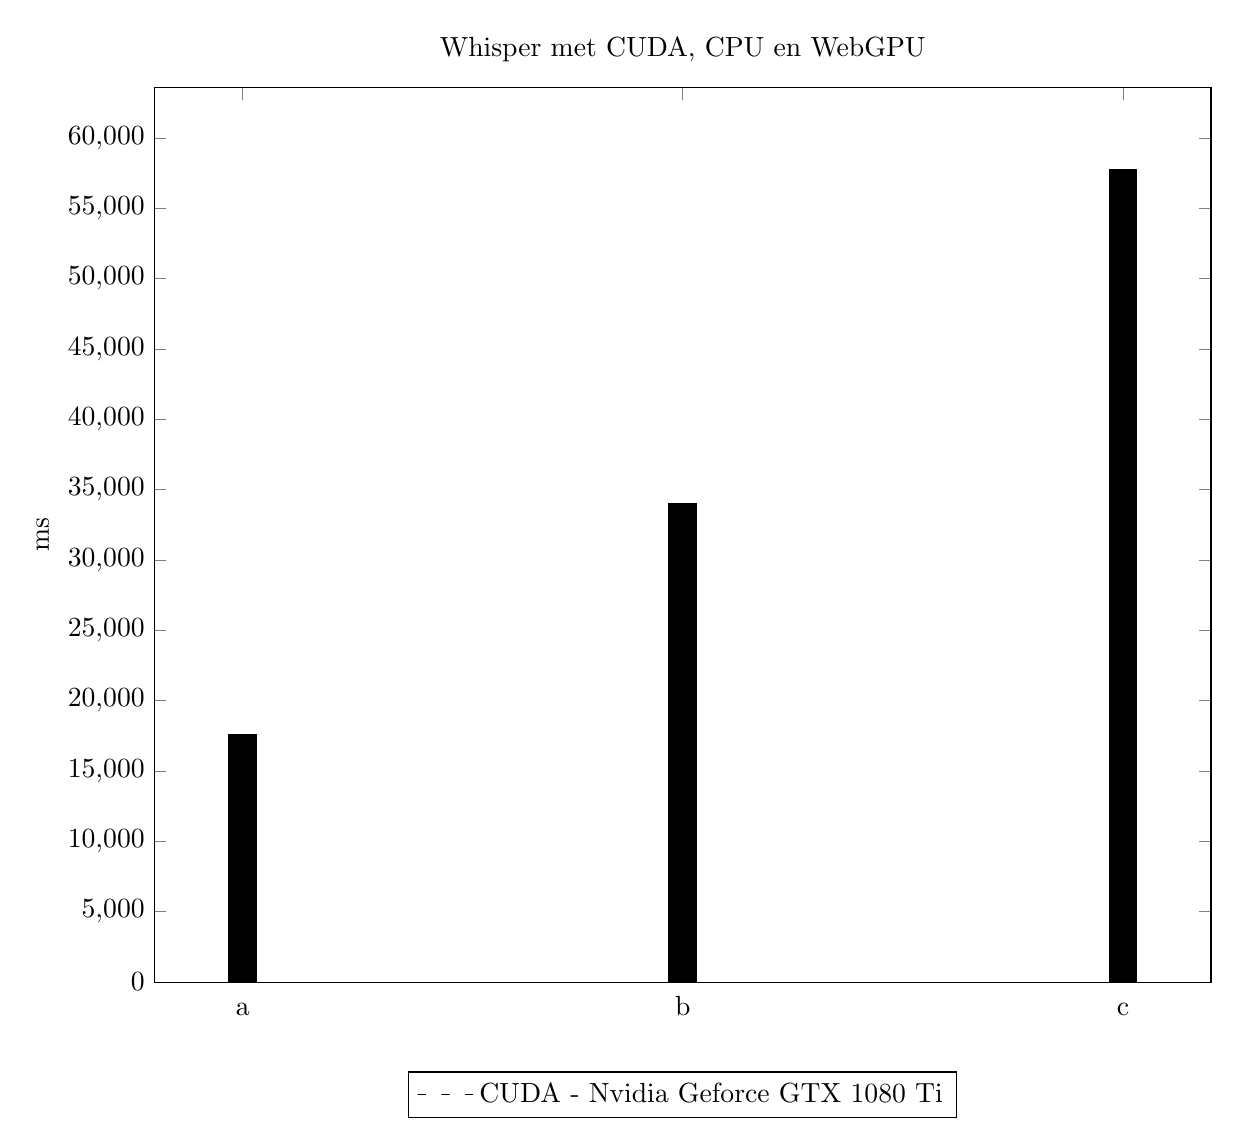
\begin{tikzpicture}

    \begin{axis}[
        title={Whisper met CUDA, CPU en WebGPU},
        symbolic x coords={a,b,c,d,e,f,g,h,i},
        xtick={a,b,c,d,e,f,g,h,i},  % Use this to decide which tickmarks to print
        xticklabel style={text height=2ex}, % This aligns all letters on the same line, if it is missing, 'a' and 'b' are at different heights
        ymin=0,
        scaled y ticks=false,
        ylabel=ms,
        legend style={at={(0.5,-0.1)},
        anchor=north,legend columns=-1},
    ]
        \addplot[ybar,fill] coordinates {
        (a,17602.3325)
        (b,34039.00)
        (c,57788.052)
        };
        \legend{CUDA - Nvidia Geforce GTX 1080 Ti,CPU - Intel Core i9,CPU - Xeon E5-2680 V2}
    \end{axis}

\end{tikzpicture}